\documentclass[]{article}
\usepackage{lmodern}
\usepackage{amssymb,amsmath}
\usepackage{ifxetex,ifluatex}
\usepackage{fixltx2e} % provides \textsubscript
\ifnum 0\ifxetex 1\fi\ifluatex 1\fi=0 % if pdftex
  \usepackage[T1]{fontenc}
  \usepackage[utf8]{inputenc}
\else % if luatex or xelatex
  \ifxetex
    \usepackage{mathspec}
    \usepackage{xltxtra,xunicode}
  \else
    \usepackage{fontspec}
  \fi
  \defaultfontfeatures{Mapping=tex-text,Scale=MatchLowercase}
  \newcommand{\euro}{€}
\fi
% use upquote if available, for straight quotes in verbatim environments
\IfFileExists{upquote.sty}{\usepackage{upquote}}{}
% use microtype if available
\IfFileExists{microtype.sty}{%
\usepackage{microtype}
\UseMicrotypeSet[protrusion]{basicmath} % disable protrusion for tt fonts
}{}
\usepackage[margin=1in]{geometry}
\usepackage{color}
\usepackage{fancyvrb}
\newcommand{\VerbBar}{|}
\newcommand{\VERB}{\Verb[commandchars=\\\{\}]}
\DefineVerbatimEnvironment{Highlighting}{Verbatim}{commandchars=\\\{\}}
% Add ',fontsize=\small' for more characters per line
\usepackage{framed}
\definecolor{shadecolor}{RGB}{248,248,248}
\newenvironment{Shaded}{\begin{snugshade}}{\end{snugshade}}
\newcommand{\KeywordTok}[1]{\textcolor[rgb]{0.13,0.29,0.53}{\textbf{{#1}}}}
\newcommand{\DataTypeTok}[1]{\textcolor[rgb]{0.13,0.29,0.53}{{#1}}}
\newcommand{\DecValTok}[1]{\textcolor[rgb]{0.00,0.00,0.81}{{#1}}}
\newcommand{\BaseNTok}[1]{\textcolor[rgb]{0.00,0.00,0.81}{{#1}}}
\newcommand{\FloatTok}[1]{\textcolor[rgb]{0.00,0.00,0.81}{{#1}}}
\newcommand{\CharTok}[1]{\textcolor[rgb]{0.31,0.60,0.02}{{#1}}}
\newcommand{\StringTok}[1]{\textcolor[rgb]{0.31,0.60,0.02}{{#1}}}
\newcommand{\CommentTok}[1]{\textcolor[rgb]{0.56,0.35,0.01}{\textit{{#1}}}}
\newcommand{\OtherTok}[1]{\textcolor[rgb]{0.56,0.35,0.01}{{#1}}}
\newcommand{\AlertTok}[1]{\textcolor[rgb]{0.94,0.16,0.16}{{#1}}}
\newcommand{\FunctionTok}[1]{\textcolor[rgb]{0.00,0.00,0.00}{{#1}}}
\newcommand{\RegionMarkerTok}[1]{{#1}}
\newcommand{\ErrorTok}[1]{\textbf{{#1}}}
\newcommand{\NormalTok}[1]{{#1}}
\usepackage{graphicx}
\makeatletter
\def\maxwidth{\ifdim\Gin@nat@width>\linewidth\linewidth\else\Gin@nat@width\fi}
\def\maxheight{\ifdim\Gin@nat@height>\textheight\textheight\else\Gin@nat@height\fi}
\makeatother
% Scale images if necessary, so that they will not overflow the page
% margins by default, and it is still possible to overwrite the defaults
% using explicit options in \includegraphics[width, height, ...]{}
\setkeys{Gin}{width=\maxwidth,height=\maxheight,keepaspectratio}
\ifxetex
  \usepackage[setpagesize=false, % page size defined by xetex
              unicode=false, % unicode breaks when used with xetex
              xetex]{hyperref}
\else
  \usepackage[unicode=true]{hyperref}
\fi
\hypersetup{breaklinks=true,
            bookmarks=true,
            pdfauthor={Sebri, JcB},
            pdftitle={Questionnaire étudiant},
            colorlinks=true,
            citecolor=blue,
            urlcolor=blue,
            linkcolor=magenta,
            pdfborder={0 0 0}}
\urlstyle{same}  % don't use monospace font for urls
\setlength{\parindent}{0pt}
\setlength{\parskip}{6pt plus 2pt minus 1pt}
\setlength{\emergencystretch}{3em}  % prevent overfull lines
\setcounter{secnumdepth}{5}

%%% Use protect on footnotes to avoid problems with footnotes in titles
\let\rmarkdownfootnote\footnote%
\def\footnote{\protect\rmarkdownfootnote}

%%% Change title format to be more compact
\usepackage{titling}

% Create subtitle command for use in maketitle
\newcommand{\subtitle}[1]{
  \posttitle{
    \begin{center}\large#1\end{center}
    }
}

\setlength{\droptitle}{-2em}
  \title{Questionnaire étudiant}
  \pretitle{\vspace{\droptitle}\centering\huge}
  \posttitle{\par}
  \author{Sebri, JcB}
  \preauthor{\centering\large\emph}
  \postauthor{\par}
  \predate{\centering\large\emph}
  \postdate{\par}
  \date{19/02/2015}



\begin{document}

\maketitle


{
\hypersetup{linkcolor=black}
\setcounter{tocdepth}{2}
\tableofcontents
}
Version du: \textbf{Wed Jul 1 18:13:21 2015}

\section{Questionnaire étudiant}\label{questionnaire-etudiant}

\begin{verbatim}
 [1] "Etab"    "Etud"    "Q1"      "Q2.1"    "Q2.2"    "Q2.3"    "Q2.4"   
 [8] "Q2.5"    "Q2.6"    "Q2.7"    "Q3.1tpc" "Q3.2sp"  "Q3.3tab" "Q3.4ord"
[15] "Q4.1"    "Q4.2"    "Q4.3"    "Q4.4"    "Q4.5"    "Q4.6"    "Q4.7"   
[22] "Q4.8"    "Q4.9"    "Q4.10"   "Q4.11"   "Q4.12"   "Q4.13"   "Q4.14"  
[29] "Q4.15"   "Q4.16"   "Q5"      "Q6"      "Q7.1"    "Q7.2"    "Q7.3"   
[36] "Q7.4"    "Q7.5"    "Q7.6"    "Q7.7"    "Q7.8"    "Q7.9"    "Q7.10"  
[43] "Q7.11"   "Q7.12"   "Q7.13"   "Q7.14"   "Q7.15"   "Q7.16"   "Q8"     
[50] "Q9"      "Q10"     "Q11"    
\end{verbatim}

Le fichier comporte:

\begin{itemize}
\itemsep1pt\parskip0pt\parsep0pt
\item
  1446 lignes
\item
  52 variables
\end{itemize}

\subsection{Etablissements
participant:}\label{etablissements-participant}

\begin{verbatim}
  B1   B2   C1   C2   C3   E1   H1   H2 HUS1 HUS2 HUS3   M1   M2  Sa1  SV1 
  43   54  120  127  110   58   56   51  162   60  131  146  123   42   79 
 SV2 
  84 
\end{verbatim}

\begin{figure}[htbp]
\centering
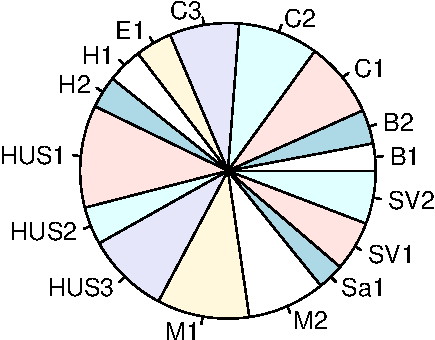
\includegraphics{qs_etudiants_files/figure-latex/participants-1.pdf}
\end{figure}

\subsection{Age}\label{age}

\begin{verbatim}
   Min. 1st Qu.  Median    Mean 3rd Qu.    Max.    NA's 
   17.0    20.0    22.0    24.1    25.0    53.0      27 
\end{verbatim}

\begin{figure}[htbp]
\centering
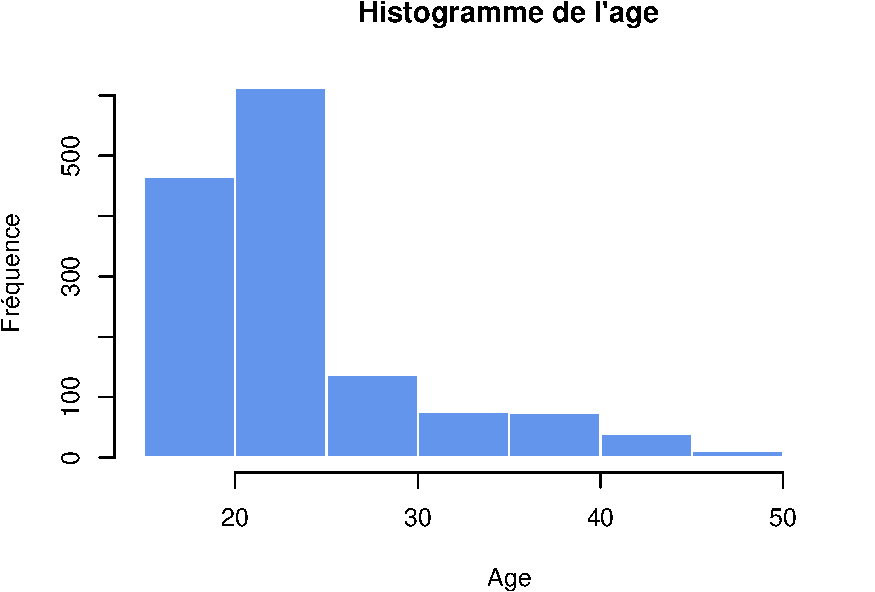
\includegraphics{qs_etudiants_files/figure-latex/age-1.pdf}
\end{figure}

\subsubsection{Générations}\label{generations}

\begin{Shaded}
\begin{Highlighting}[]
\CommentTok{# génération}
\CommentTok{# Z = 15 à 20 ans}
\CommentTok{# Y = 20 à 35 ans}
\CommentTok{# X > 35 ans}

\NormalTok{age <-}\StringTok{ }\KeywordTok{c}\NormalTok{(}\DecValTok{15}\NormalTok{, }\DecValTok{20}\NormalTok{, }\DecValTok{35}\NormalTok{, }\DecValTok{60}\NormalTok{)}
\NormalTok{g <-}\StringTok{ }\KeywordTok{cut}\NormalTok{(d1$Q11, age)}
\KeywordTok{summary}\NormalTok{(g)}
\end{Highlighting}
\end{Shaded}

\begin{verbatim}
## (15,20] (20,35] (35,60]    NA's 
##     466     826     127      27
\end{verbatim}

\begin{Shaded}
\begin{Highlighting}[]
\NormalTok{g2 <-}\StringTok{ }\KeywordTok{cut}\NormalTok{(d1$Q11, age, }\DataTypeTok{labels =} \KeywordTok{c}\NormalTok{(}\StringTok{"Z"}\NormalTok{, }\StringTok{"Y"}\NormalTok{, }\StringTok{"X"}\NormalTok{))}
\KeywordTok{summary}\NormalTok{(g2)}
\end{Highlighting}
\end{Shaded}

\begin{verbatim}
##    Z    Y    X NA's 
##  466  826  127   27
\end{verbatim}

\begin{Shaded}
\begin{Highlighting}[]
\CommentTok{# ajout d'une colonne GENERATION}
\NormalTok{d1$GENERATION <-}\StringTok{ }\NormalTok{g2}
\KeywordTok{factor2table}\NormalTok{(d1$GENERATION)}
\end{Highlighting}
\end{Shaded}

\begin{verbatim}
##                 Z      Y      X  NA's
## nombre     466.00 826.00 127.00 27.00
## proportion  32.23  57.12   8.78  1.87
\end{verbatim}

\begin{Shaded}
\begin{Highlighting}[]
\KeywordTok{barplot}\NormalTok{(}\KeywordTok{summary}\NormalTok{(d1$GENERATION), }\DataTypeTok{xlab =} \StringTok{"Génération"}\NormalTok{, }\DataTypeTok{ylab =} \StringTok{"nombre"}\NormalTok{, }\DataTypeTok{main =} \StringTok{"Répartition des générations au sein des étudiants"}\NormalTok{)}
\end{Highlighting}
\end{Shaded}

\begin{figure}[htbp]
\centering
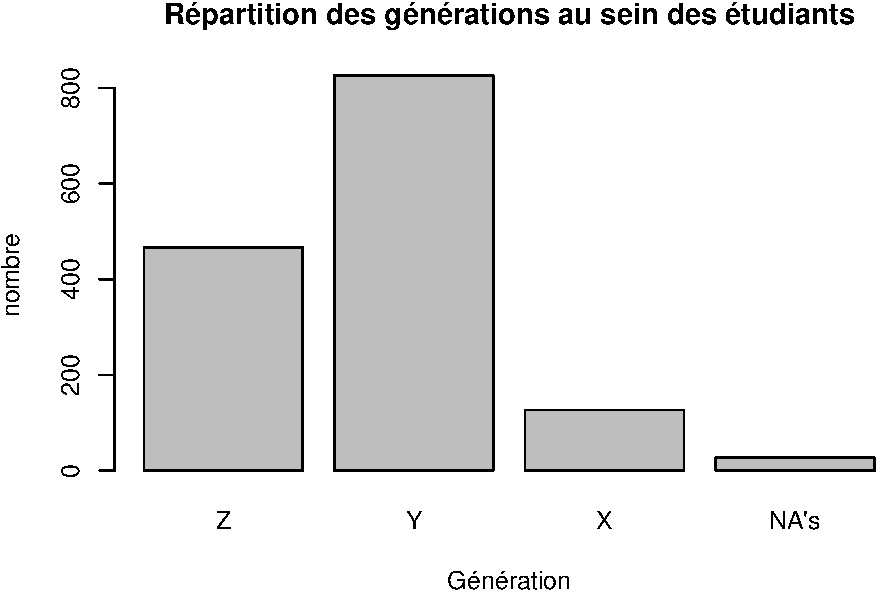
\includegraphics{qs_etudiants_files/figure-latex/generation-1.pdf}
\end{figure}

\subsection{Sexe}\label{sexe}

\begin{verbatim}
   F    H   na NA's 
1218  210    1   17 
\end{verbatim}

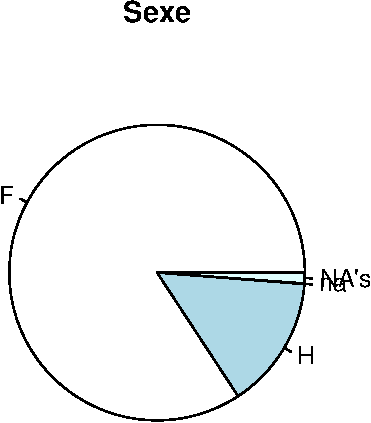
\includegraphics{qs_etudiants_files/figure-latex/sexe-1.pdf} Test de la
routine \textbf{factor2table}

\begin{Shaded}
\begin{Highlighting}[]
\NormalTok{f <-}\StringTok{ }\KeywordTok{factor2table}\NormalTok{(d1$Q10, }\DataTypeTok{digit=}\DecValTok{2}\NormalTok{, }\DataTypeTok{col=}\KeywordTok{c}\NormalTok{(}\StringTok{"femmes"}\NormalTok{,}\StringTok{"hommes"}\NormalTok{,}\StringTok{"inconnu"}\NormalTok{))}
\NormalTok{f}
\end{Highlighting}
\end{Shaded}

\begin{verbatim}
##             femmes hommes inconnu
## nombre     1218.00 210.00   18.00
## proportion   84.23  14.52    1.24
\end{verbatim}

Sous forme de tableau avec \textbf{kable}:

\begin{table}

\caption{Sexe des participants}
\begin{tabular}{l|r|r|r}
\hline
  & femmes & hommes & inconnu\\
\hline
nombre & 1218.00 & 210.00 & 18.00\\
\hline
proportion & 84.23 & 14.52 & 1.24\\
\hline
\end{tabular}
\end{table}

Sous forme de tableau avec \textbf{xtable}:

\% latex table generated in R 3.1.3 by xtable 1.7-4 package \% Wed Jul 1
18:13:25 2015

\begin{table}[ht]
\centering
\begin{tabular}{rrrr}
  \hline
 & femmes & hommes & inconnu \\ 
  \hline
nombre & 1218.00 & 210.00 & 18.00 \\ 
  proportion & 84.23 & 14.52 & 1.24 \\ 
   \hline
\end{tabular}
\caption{Sexe des participants} 
\label{sexe}
\end{table}

Pie chart
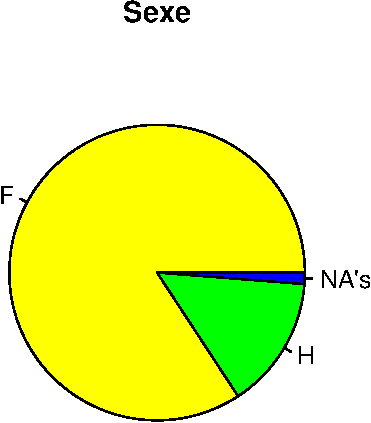
\includegraphics{qs_etudiants_files/figure-latex/pie_sexe-1.pdf}

\subsection{Age et sexe}\label{age-et-sexe}

L'age des hommes et des femmes sont-ils identiques ? On part de
l'hypothèse qu'il n'y a à priori de différence d'age entre les hommes et
les femmes (on appelle cela l'hypothèse nulle ou H0). Si cette hypothèse
est vraie, la différence des moyennes des ages entre les hommes et les
femmes devrait être nulle. En pratique cette différence est rarement
exactement égale à 0 et le problème est de savoir si le chiffre obtenu
est assimilable à 0 ou si on contraire il est trop important pourqu'on
puisse se livrer à cette assimilation, auquel cas on est obligé de
renoncer à l'hypothèse nulle et accepter l'hypothèse alternative: l'age
des hommes est en moyenne différent de celui des femmes. Pour répondre à
la question, on pratique un test statistique pour lequel on défini un
écart par rappport à 0. Si le résultat du test tombe dans l'intervalle
on admet que la différence de moyenne est assimilable à 0 et on accepte
l'hypothèse nulle: pas de différence entre les groupes. Sinon on la
recherche. Bien sûr, plus on défini un intervalle important, plus on
augmente le risque de se tromper en affirmant qu'il n'y a pas de
différence entre les moyennes. C'est ce qu'on appelle le risque de
première espèce ou alpha. Dans les science de la santé, ce risque est
fixé conssenssuellement (et arbitrairement) à 5\% = 5/100 = 0.05 et
généralement rapporté sous la forme p = 0.05 C'est à dire que j'admet H0
(pas de différence) en prenant le risque conssenti de me tromper dans
5\% des cas. En pratique les logiciels calculent la probabilité exacte
d'observer par hasard une telle différence entre les deux groupes. Si
cette probabilité est supérieure à 0.05 (cad comprise entre 0.05 et 1)
on considère que la différence entre les moyennes est un artefact lié au
fluctuation d'échantillonnage et qu'en réalité il n'y a pas de
différence entre les groupes. Si au contraire, la probabilité exacte est
inférieure à 0.05, on admet qu'elle n'est pas due au hasard et on est
obligé d'admettre qu'il y a bien une différence entre les deux groupes.
On voit par là le côté arbitraire du petit p, mais il est considéré dans
toutes les publications comme un chiffre magique\ldots{}

Il existe de nombreux tests statistiques. Pour répondre à la question
posée, on utilise le test t de Student qui s'applique si:

\begin{itemize}
\itemsep1pt\parskip0pt\parsep0pt
\item
  on ne compare que 2 groupes (c'est le cas)
\item
  la variable d'intérêt (ici l'age) suit une loi normale (on va admettre
  que oui) dans les 2 groupes
\item
  la variance (moyenne des écarts à la moyenne) des 2 groupes est égale
  (si ce n'est pas le cas, on peut utiliser une variante de test de
  Student appelée test de Welch).
\end{itemize}

La colonne sexe (Q10) comporte 3 valeurs: H, F et NR. Il faut éliminer
les NR en les transformant en NA pour rendre le test possible

\begin{Shaded}
\begin{Highlighting}[]
\NormalTok{d1$Q10 <-}\StringTok{ }\KeywordTok{toupper}\NormalTok{(d1$Q10)}
\NormalTok{d1$Q10[d1$Q10 ==}\StringTok{ "NR"}\NormalTok{] <-}\StringTok{ }\OtherTok{NA}
\end{Highlighting}
\end{Shaded}

Puis faire le test:

\begin{Shaded}
\begin{Highlighting}[]
\NormalTok{t <-}\StringTok{ }\KeywordTok{t.test}\NormalTok{(d1$Q11 ~}\StringTok{ }\NormalTok{d1$Q10, }\DataTypeTok{var.equal =} \OtherTok{TRUE}\NormalTok{)}
\NormalTok{t}
\end{Highlighting}
\end{Shaded}

\begin{verbatim}
## 
##  Two Sample t-test
## 
## data:  d1$Q11 by d1$Q10
## t = -3.7563, df = 1415, p-value = 0.0001795
## alternative hypothesis: true difference in means is not equal to 0
## 95 percent confidence interval:
##  -2.7497617 -0.8630462
## sample estimates:
## mean in group F mean in group H 
##        23.82645        25.63285
\end{verbatim}

\begin{Shaded}
\begin{Highlighting}[]
\NormalTok{p.t <-}\StringTok{ }\NormalTok{t$p.value}
\end{Highlighting}
\end{Shaded}

On voit que la probabilité exacte d'observer par hasard une telle
différence entre les moyennes est égale à 0.0001795. Cette probabilité
est très inférieure à 0.05 et donc on rejette l'hypothèse d'égalité des
ages. En moyenne, pour cet échantillon, les étudiants hommes sont plus
agés que les étudiantes et cette différence est statistiquement
significative.

Comme on peut avoir un doute sérieux sur la normalité de l'age (voir le
graphique des ages ci-dessus), on réalise un test non paramétrique,
c'est à dire qui ne fait pas d'hypothèse sur la façon dont la variable
est distribuée. Dans le cas particulier on utilise le test de Wilcoxon
qui est l'équivalent non paramétrique du test de Student:

\begin{Shaded}
\begin{Highlighting}[]
\KeywordTok{wilcox.test}\NormalTok{(d1$Q11 ~}\StringTok{ }\NormalTok{d1$Q10)}
\end{Highlighting}
\end{Shaded}

\begin{verbatim}
## 
##  Wilcoxon rank sum test with continuity correction
## 
## data:  d1$Q11 by d1$Q10
## W = 97211, p-value = 0.0000002159
## alternative hypothesis: true location shift is not equal to 0
\end{verbatim}

On arrive à la même conclusion.

\subsection{Q1- Pour ce cours, vous avez pris des
notes}\label{q1--pour-ce-cours-vous-avez-pris-des-notes}

\begin{verbatim}
             ordi papier    pas     X
nombre     410.00 720.00 232.00 84.00
proportion  28.35  49.79  16.04  5.81
\end{verbatim}

\begin{figure}[htbp]
\centering
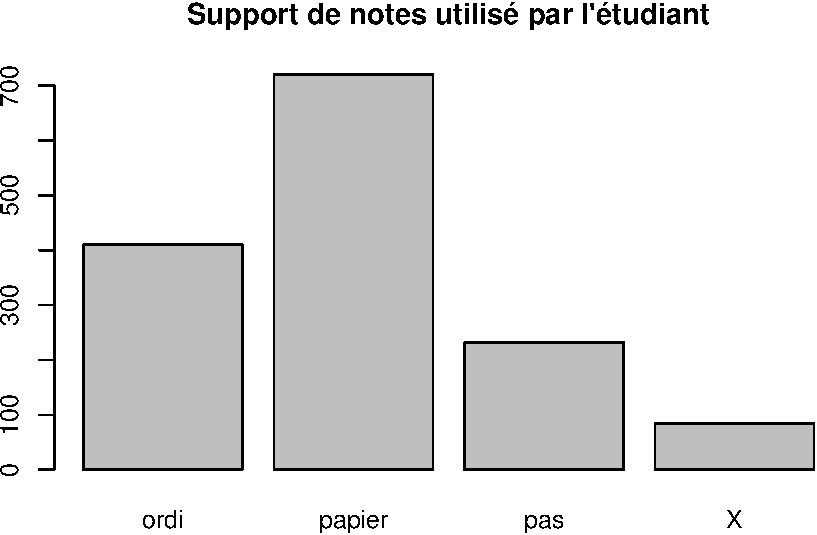
\includegraphics{qs_etudiants_files/figure-latex/Q1-1.pdf}
\end{figure}

\subsection{Q2- Pendant ce cours, vous avez complété la prise de notes
par (plusieurs réponses
possibles)}\label{q2--pendant-ce-cours-vous-avez-complete-la-prise-de-notes-par-plusieurs-reponses-possibles}

La variable Q2.5 est anormale. Il ne peut y avoir dans la même colonne
du texte et des nombres. La colonne ne peut contenir que 1 ou NA. Créer
une colnne supplémentaire pour le texte. Par ex. Q2-7.

\begin{figure}[htbp]
\centering
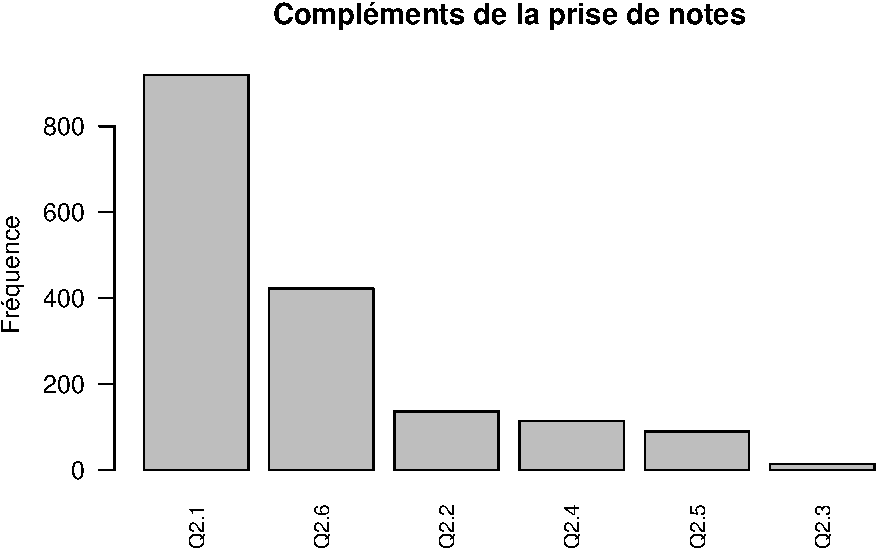
\includegraphics{qs_etudiants_files/figure-latex/unnamed-chunk-3-1.pdf}
\end{figure}

\begin{verbatim}
              0       1      2     3    4
nombre     8.00 1201.00 218.00 17.00 2.00
proportion 0.55   83.06  15.08  1.18 0.14
\end{verbatim}

\begin{figure}[htbp]
\centering
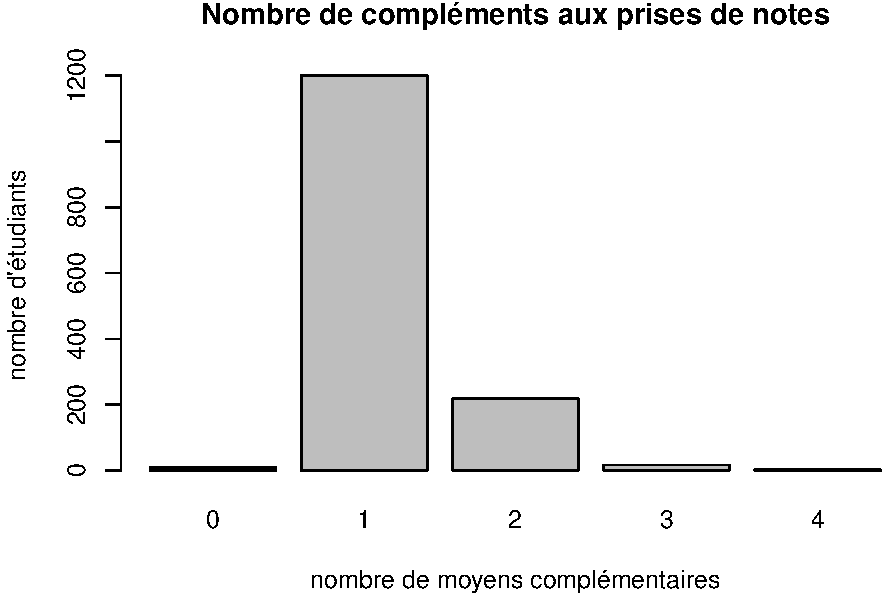
\includegraphics{qs_etudiants_files/figure-latex/unnamed-chunk-3-2.pdf}
\end{figure}

\subsection{Q3- Quels sont les outils numériques que vous aviez avec
vous pendant ce cours? (plusieurs réponses
possibles)}\label{q3--quels-sont-les-outils-numeriques-que-vous-aviez-avec-vous-pendant-ce-cours-plusieurs-reponses-possibles}

Colonnes 11 à 14

4 types d'outils:

\begin{itemize}
\itemsep1pt\parskip0pt\parsep0pt
\item
  téléphone portable classique (tpc)
\item
  smartphone (sp)
\item
  tablette (tab)
\item
  ordinateur portable (ord)
\end{itemize}

ces outils sont-ils disponibles: non, oui, et si oui où:

\begin{itemize}
\itemsep1pt\parskip0pt\parsep0pt
\item
  sur la table= ot
\item
  dans mon sac ou ma poche= osp
\end{itemize}

\begin{figure}[htbp]
\centering
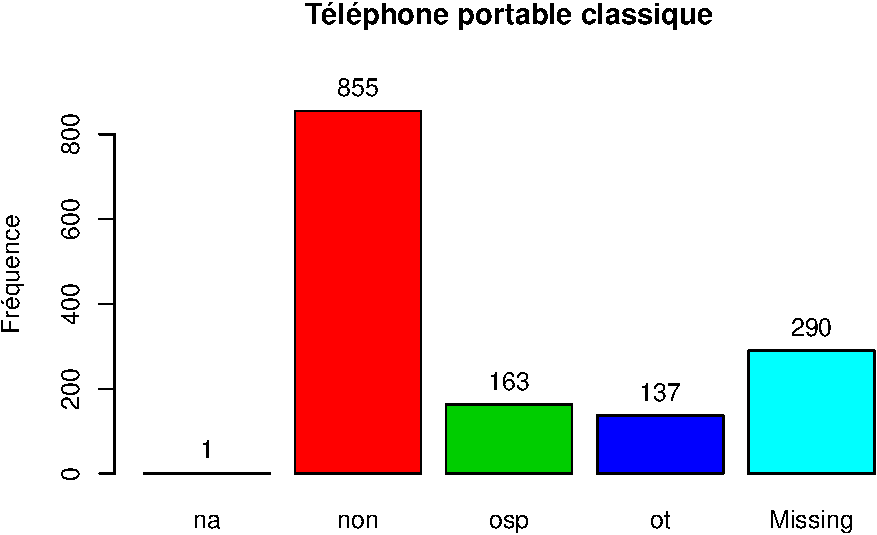
\includegraphics{qs_etudiants_files/figure-latex/outils-1.pdf}
\end{figure}

\begin{verbatim}
d1$Q3.1tpc : 
        Frequency   %(NA+)   %(NA-)
na              1      0.1      0.1
non           855     59.1     74.0
osp           163     11.3     14.1
ot            137      9.5     11.9
<NA>          290     20.1      0.0
  Total      1446    100.0    100.0
\end{verbatim}

\begin{figure}[htbp]
\centering
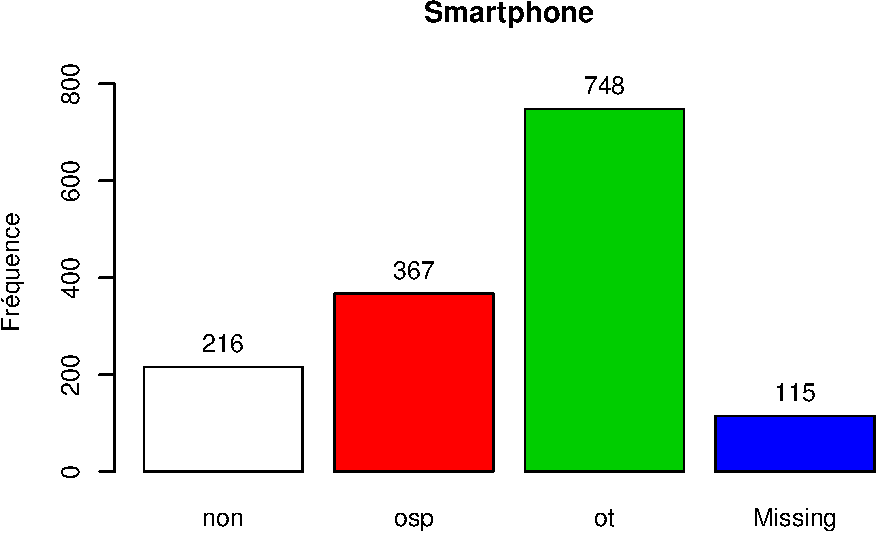
\includegraphics{qs_etudiants_files/figure-latex/outils-2.pdf}
\end{figure}

\begin{verbatim}
d1$Q3.2sp : 
        Frequency   %(NA+)   %(NA-)
non           216     14.9     16.2
osp           367     25.4     27.6
ot            748     51.7     56.2
<NA>          115      8.0      0.0
  Total      1446    100.0    100.0
\end{verbatim}

\begin{figure}[htbp]
\centering
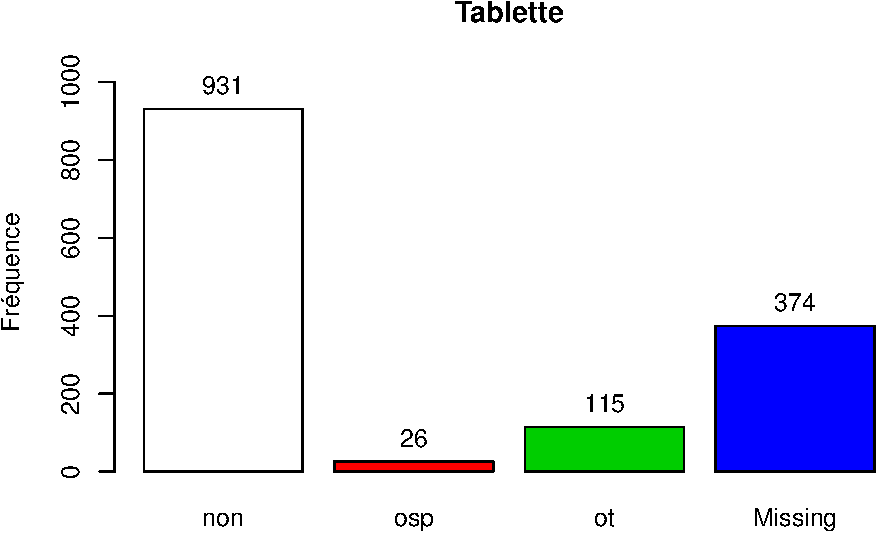
\includegraphics{qs_etudiants_files/figure-latex/outils-3.pdf}
\end{figure}

\begin{verbatim}
d1$Q3.3tab : 
        Frequency   %(NA+)   %(NA-)
non           931     64.4     86.8
osp            26      1.8      2.4
ot            115      8.0     10.7
<NA>          374     25.9      0.0
  Total      1446    100.0    100.0
\end{verbatim}

\begin{figure}[htbp]
\centering
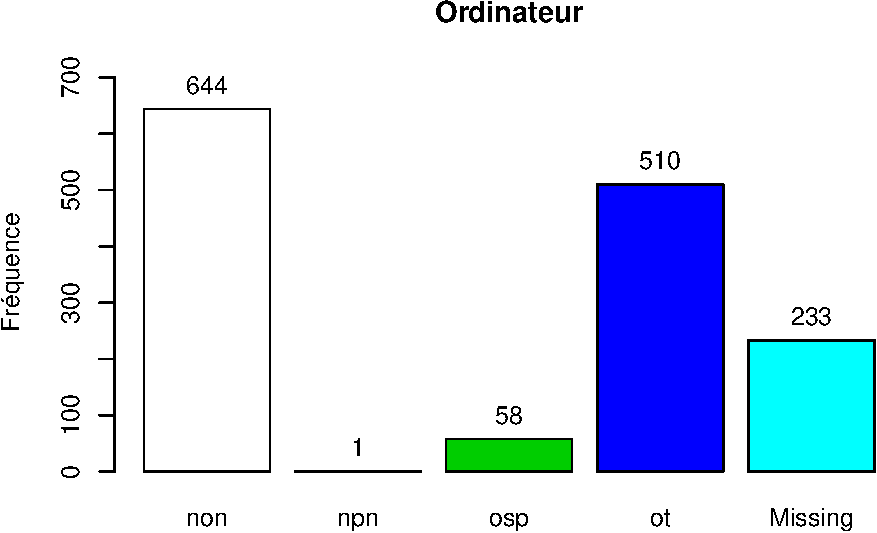
\includegraphics{qs_etudiants_files/figure-latex/outils-4.pdf}
\end{figure}

\begin{verbatim}
d1$Q3.4ord : 
        Frequency   %(NA+)   %(NA-)
non           644     44.5     53.1
npn             1      0.1      0.1
osp            58      4.0      4.8
ot            510     35.3     42.0
<NA>          233     16.1      0.0
  Total      1446    100.0    100.0
\end{verbatim}

\#\#\# Résultats:

\begin{itemize}
\itemsep1pt\parskip0pt\parsep0pt
\item
  nombre de personnes n'ayant pas répondu à chacune des questions: voir
  table \ref{lab.tnr} pp \pageref{lab.tnr}
\end{itemize}

\% latex table generated in R 3.1.3 by xtable 1.7-4 package \% Wed Jul 1
18:13:33 2015

\begin{table}[ht]
\centering
\begin{tabular}{rrrrr}
  \hline
 & Q3.1tpc & Q3.2sp & Q3.3tab & Q3.4ord \\ 
  \hline
nombre & 290.00 & 115.00 & 374.00 & 233.00 \\ 
   \%  & 20.06 & 7.95 & 25.86 & 16.11 \\ 
   \hline
\end{tabular}
\caption{Ne réponsent à aucune des 4 questions} 
\label{lab.tnr}
\end{table}

\begin{itemize}
\item
  ont un tpc: 300 (20.75 \%)
\item
  ont un smartphone: 1115 (77.11 \%)
\item
  ont un tpc ET un smartphone: 106 (7.33 \%)
\item
  ont un tpc OU un smartphone: 1309 (90.53 \%)
\item
  n'ont NI tcp NI sp: 137 (9.47 \%)
\item
  ont une tablette: 141 (9.75 \%)
\item
  ont un ordinateur portable: 568 (39.28 \%)
\item
  ont une tablette ET un ordinateur: 21 (1.45 \%)
\item
  ont une tablette OU un ordinateur: 688 (47.58 \%)
\item
  n'ont NI ordi, NI tablette: 757 (52.35 \%)
\item
  ont un ordinateur ET un smartphone: 475 (32.85 \%)
\item
  ne réponsent à aucune des 4 questions: 11 (0.76 \%)
\end{itemize}

\subsubsection{selon la généation}\label{selon-la-geneation}

\paragraph{portable classique}\label{portable-classique}

\begin{verbatim}
##      
##         Z   Y   X
##   na    0   0   1
##   non 299 495  46
##   osp  36  77  47
##   ot   34  90  11
\end{verbatim}

\begin{verbatim}
##   na  non  oui NA's 
##    1  855  300  290
\end{verbatim}

\begin{verbatim}
##               génération
## possède un tpc   Z   Y   X
##            na    0   0   1
##            non 299 495  46
##            oui  70 167  58
\end{verbatim}

\begin{verbatim}
## Warning in chisq.test(table(tpc, d1$GENERATION)): Chi-squared approximation
## may be incorrect
\end{verbatim}

\begin{verbatim}
## 
##  Pearson's Chi-squared test
## 
## data:  table(tpc, d1$GENERATION)
## X-squared = 67.0208, df = 4, p-value = 9.651e-14
\end{verbatim}

\paragraph{smartphone}\label{smartphone}

\begin{verbatim}
##      
##         Z   Y   X
##   non  44 108  57
##   osp 153 186  25
##   ot  254 466  15
\end{verbatim}

\begin{verbatim}
##  non  oui NA's 
##  216 1115  115
\end{verbatim}

\begin{verbatim}
##              génération
## possède un sp   Z   Y   X
##           non  44 108  57
##           oui 407 652  40
\end{verbatim}

\begin{verbatim}
## 
##  Pearson's Chi-squared test
## 
## data:  table(sp, d1$GENERATION)
## X-squared = 147.0316, df = 2, p-value < 2.2e-16
\end{verbatim}

\paragraph{tablette}\label{tablette}

\begin{verbatim}
##      
##         Z   Y   X
##   non 315 518  81
##   osp   8  13   4
##   ot   37  76   2
\end{verbatim}

\begin{verbatim}
##  non  oui NA's 
##  931  141  374
\end{verbatim}

\begin{verbatim}
##               génération
## possède un tab   Z   Y   X
##            non 315 518  81
##            oui  45  89   6
\end{verbatim}

\begin{verbatim}
## 
##  Pearson's Chi-squared test
## 
## data:  table(tab, d1$GENERATION)
## X-squared = 4.2748, df = 2, p-value = 0.118
\end{verbatim}

Pas de différence entre les génération

\paragraph{ordinateur}\label{ordinateur}

\begin{verbatim}
##      
##         Z   Y   X
##   non 189 374  68
##   npn   0   0   1
##   osp  15  38   3
##   ot  202 278  21
\end{verbatim}

\begin{verbatim}
##  non  oui NA's 
##  645  568  233
\end{verbatim}

\begin{verbatim}
##               génération
## possède un ord   Z   Y   X
##            non 189 374  69
##            oui 217 316  24
\end{verbatim}

\begin{verbatim}
## 
##  Pearson's Chi-squared test
## 
## data:  table(ord, d1$GENERATION)
## X-squared = 23.945, df = 2, p-value = 0.000006316
\end{verbatim}

\begin{verbatim}
## [1] "tableau attendu si H0 vraie"
\end{verbatim}

\begin{verbatim}
##      
## ord          Z       Y        X
##   non 215.8049 366.762 49.43314
##   oui 190.1951 323.238 43.56686
\end{verbatim}

\begin{verbatim}
## [1] "différence observé - attendu"
\end{verbatim}

\begin{verbatim}
##      
## ord            Z          Y          X
##   non -26.804878   7.238015  19.566863
##   oui  26.804878  -7.238015 -19.566863
\end{verbatim}

\subsubsection{création d'une colonne moyens de
COMmunication:}\label{creation-dune-colonne-moyens-de-communication}

Possédez-vous un tpc ou un smartphone:

\begin{verbatim}
##  non  oui NA's 
##   91 1312   43
\end{verbatim}

Selon la génération:

\begin{verbatim}
##    
##     non oui
##   Z  14 445
##   Y  45 756
##   X  27  91
\end{verbatim}

\begin{verbatim}
##    
##       non   oui
##   Z  3.05 96.95
##   Y  5.62 94.38
##   X 22.88 77.12
\end{verbatim}

\begin{verbatim}
## 
##  Pearson's Chi-squared test
## 
## data:  table(d1$GENERATION, d1$COM)
## X-squared = 64.3581, df = 2, p-value = 1.059e-14
\end{verbatim}

\subsection{Q4- Pendant ce cours (en dehors des temps de pause
éventuels), vous avez utilisé votre téléphone pour (plusieurs réponses
possibles):}\label{q4--pendant-ce-cours-en-dehors-des-temps-de-pause-eventuels-vous-avez-utilise-votre-telephone-pour-plusieurs-reponses-possibles}

question 15 à 30

\begin{Shaded}
\begin{Highlighting}[]
\NormalTok{d1 <-}\StringTok{ }\KeywordTok{read.csv}\NormalTok{(}\KeywordTok{paste0}\NormalTok{(path, file1), }\DataTypeTok{skip =} \DecValTok{1}\NormalTok{, }\DataTypeTok{stringsAsFactors =} \OtherTok{FALSE}\NormalTok{)}

\NormalTok{q4 <-}\StringTok{ }\NormalTok{d1[, }\KeywordTok{c}\NormalTok{(}\DecValTok{15}\NormalTok{:}\DecValTok{26}\NormalTok{, }\DecValTok{28}\NormalTok{:}\DecValTok{30}\NormalTok{)]}
\NormalTok{q4 <-}\StringTok{ }\KeywordTok{as.data.frame}\NormalTok{(}\KeywordTok{sapply}\NormalTok{(q4,gsub,}\DataTypeTok{pattern=}\StringTok{"NR"}\NormalTok{,}\DataTypeTok{replacement=}\StringTok{"NA"}\NormalTok{), }\DataTypeTok{stringsAsFactors =} \OtherTok{FALSE}\NormalTok{)}
\NormalTok{q4 <-}\StringTok{ }\KeywordTok{as.data.frame}\NormalTok{(}\KeywordTok{sapply}\NormalTok{(q4, as.integer))}
\NormalTok{a <-}\StringTok{ }\KeywordTok{apply}\NormalTok{(q4,}\DecValTok{2}\NormalTok{,sum, }\DataTypeTok{na.rm =} \OtherTok{TRUE}\NormalTok{)}
\NormalTok{x <-}\StringTok{ }\KeywordTok{barplot}\NormalTok{(}\KeywordTok{sort}\NormalTok{(a, }\DataTypeTok{decreasing =} \OtherTok{TRUE}\NormalTok{), }\DataTypeTok{las =} \DecValTok{2}\NormalTok{, }\DataTypeTok{main =} \StringTok{"Utilisation du téléphone pendant le cours"}\NormalTok{)}
\NormalTok{v <-}\StringTok{ }\KeywordTok{paste0}\NormalTok{(}\KeywordTok{sort}\NormalTok{(}\KeywordTok{round}\NormalTok{(a*}\DecValTok{100}\NormalTok{/}\KeywordTok{sum}\NormalTok{(a), }\DecValTok{2}\NormalTok{), }\DataTypeTok{decreasing =} \OtherTok{TRUE}\NormalTok{), }\StringTok{"%"}\NormalTok{)}
\KeywordTok{text}\NormalTok{(x, }\DecValTok{100}\NormalTok{, v, }\DataTypeTok{srt=}\DecValTok{90}\NormalTok{, }\DataTypeTok{cex =} \FloatTok{0.8}\NormalTok{)}
\end{Highlighting}
\end{Shaded}

\begin{figure}[htbp]
\centering
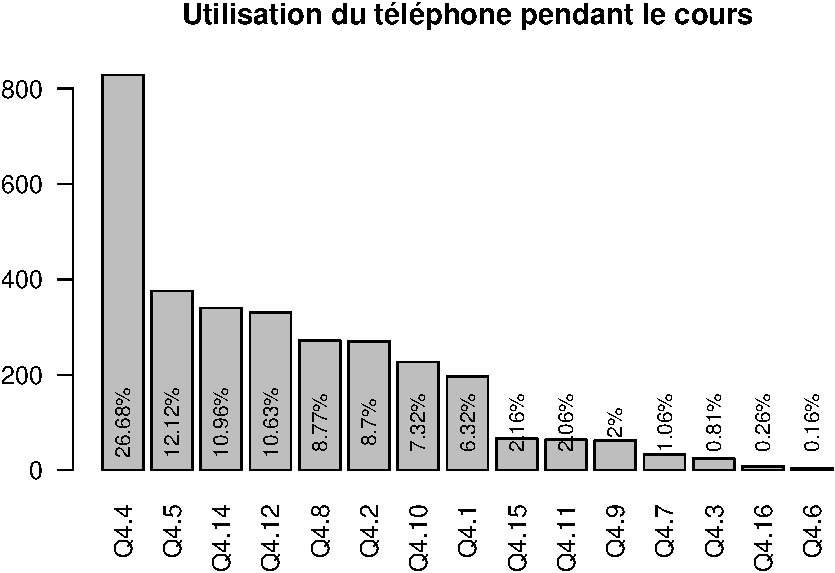
\includegraphics{qs_etudiants_files/figure-latex/Q4-1.pdf}
\end{figure}

Combien d'actions simultannément:

\begin{verbatim}
   Min. 1st Qu.  Median    Mean 3rd Qu.    Max. 
  0.000   1.000   2.000   2.146   3.000  12.000 
\end{verbatim}

\begin{verbatim}
  0   1   2   3   4   5   6   7   8  11  12 
 42 635 311 207 122  74  31  18   4   1   1 
\end{verbatim}

\begin{figure}[htbp]
\centering
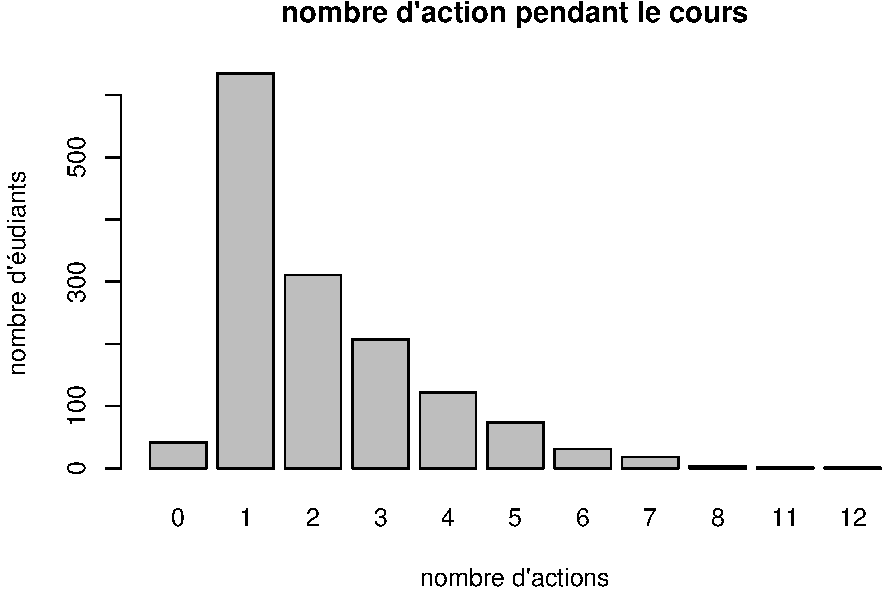
\includegraphics{qs_etudiants_files/figure-latex/actions_sim-1.pdf}
\end{figure}

\subsection{Q5- A quelle fréquence, avez-vous utilisé votre téléphone
PENDANT ce cours (en dehors des temps de pause éventuels) pour prendre
des notes ou chercher sur internet des informations au sujet du cours
?}\label{q5--a-quelle-frequence-avez-vous-utilise-votre-telephone-pendant-ce-cours-en-dehors-des-temps-de-pause-eventuels-pour-prendre-des-notes-ou-chercher-sur-internet-des-informations-au-sujet-du-cours}

question 31

\begin{verbatim}
  1X  jjs jnsp   js   na   NR  nvp  qqf   sv   tt NA's 
 136    1    9  835    6   66   11  251   64    9   58 
\end{verbatim}

\begin{figure}[htbp]
\centering
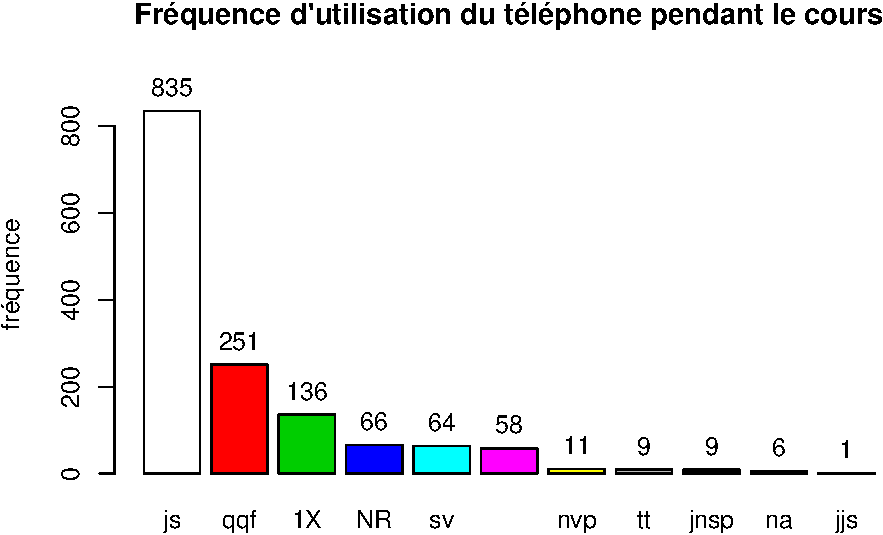
\includegraphics{qs_etudiants_files/figure-latex/utilisation-1.pdf}
\end{figure}

\begin{verbatim}
as.factor(d1$Q5) : 
        Frequency   %(NA+)   %(NA-)
js            835     57.7     60.2
qqf           251     17.4     18.1
1X            136      9.4      9.8
NR             66      4.6      4.8
sv             64      4.4      4.6
NA's           58      4.0      0.0
nvp            11      0.8      0.8
jnsp            9      0.6      0.6
tt              9      0.6      0.6
na              6      0.4      0.4
jjs             1      0.1      0.1
  Total      1446    100.0    100.0
\end{verbatim}

\subsection{Q6- A quelle fréquence, avez-vous utilisé votre téléphone
PENDANT ce cours (en dehors des temps de pause éventuels) pour faire
autre chose que prendre des notes ou chercher sur internet des
informations au sujet du
cours?}\label{q6--a-quelle-frequence-avez-vous-utilise-votre-telephone-pendant-ce-cours-en-dehors-des-temps-de-pause-eventuels-pour-faire-autre-chose-que-prendre-des-notes-ou-chercher-sur-internet-des-informations-au-sujet-du-cours}

question 32

\begin{verbatim}
  1X jnsp   js   na   NR  nvp  qqf   sv   tt NA's 
 183    5  303    3   67   16  524  242   45   58 
\end{verbatim}

\begin{figure}[htbp]
\centering
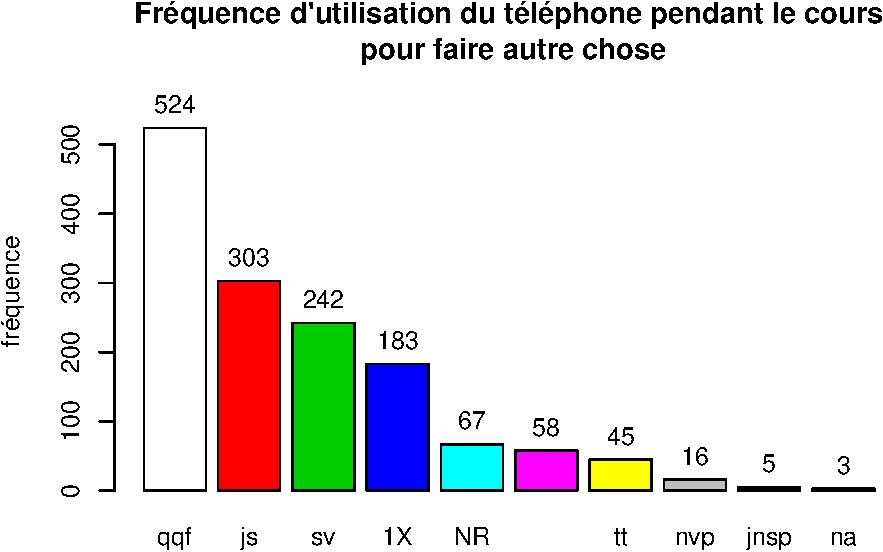
\includegraphics{qs_etudiants_files/figure-latex/utilisation2-1.pdf}
\end{figure}

\begin{verbatim}
as.factor(d1$Q6) : 
        Frequency   %(NA+)   %(NA-)
qqf           524     36.2     37.8
js            303     21.0     21.8
sv            242     16.7     17.4
1X            183     12.7     13.2
NR             67      4.6      4.8
NA's           58      4.0      0.0
tt             45      3.1      3.2
nvp            16      1.1      1.2
jnsp            5      0.3      0.4
na              3      0.2      0.2
  Total      1446    100.0    100.0
\end{verbatim}

\subsection{Q7- Pendant ce cours (en dehors des temps de pause
éventuels), vous avez utilisé votre tablette et/ ou votre ordinateur
pour (plusieurs réponses
possibles):}\label{q7--pendant-ce-cours-en-dehors-des-temps-de-pause-eventuels-vous-avez-utilise-votre-tablette-et-ou-votre-ordinateur-pour-plusieurs-reponses-possibles}

Questions 33 à 48

\begin{verbatim}
[1] "Analyse de la colonne Q7.13 (réponse libre)"
\end{verbatim}

\begin{verbatim}
                            1          cours  dessinerpaint        docmail 
          1335              1              1              1              1 
      frfiches    inscrcourse        Lemotiv           lire     notercours 
             1              1              1              3             39 
   orgdossinfo            ppt       pptcours         prepCV  reg_autr_cour 
             1              1              3              2              1 
  reg_pptander      reg-heure     reg-photos        reg-ppt regautre cours 
             1              1              1              1              1 
      regcours         regppt           shop    suivrecours        support 
             1              1              3              1              1 
 telecharcours            TFE           word           WTFE           NA's 
             1              3              1              1             36 
\end{verbatim}

\begin{verbatim}
 Q7.1  Q7.2  Q7.3  Q7.4  Q7.5  Q7.6  Q7.7  Q7.8  Q7.9 Q7.10 Q7.11 Q7.12 
   63    55    39    70     7     5    42     5    42    91   368    53 
Q7.14 Q7.15 Q7.16 
  234   640    14 
\end{verbatim}

\begin{figure}[htbp]
\centering
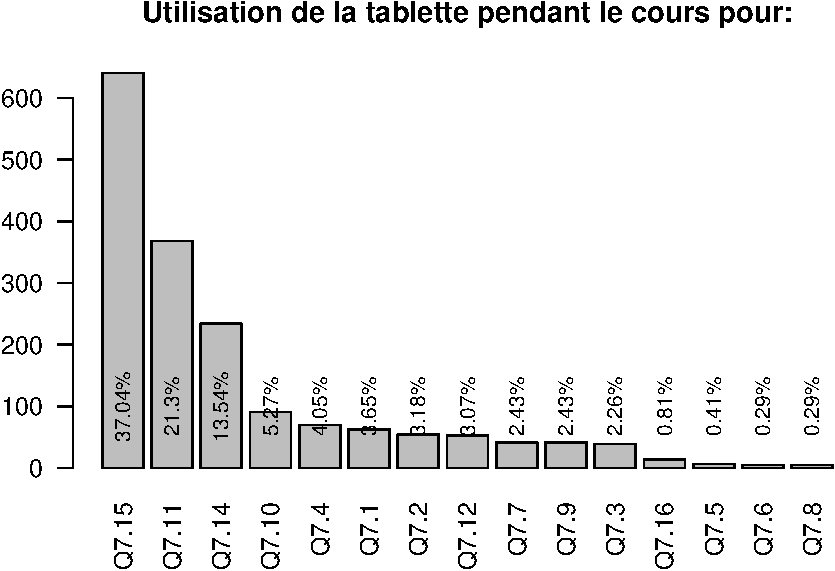
\includegraphics{qs_etudiants_files/figure-latex/q7-1.pdf}
\end{figure}

\subsection{Q8- A quelle fréquence, avez-vous utilisé votre tablette,
et/ ou votre ordinateur PENDANT ce cours (en dehors des temps de pause
éventuels) pour prendre des notes ou chercher sur internet des
informations au sujet du cours
?}\label{q8--a-quelle-frequence-avez-vous-utilise-votre-tablette-et-ou-votre-ordinateur-pendant-ce-cours-en-dehors-des-temps-de-pause-eventuels-pour-prendre-des-notes-ou-chercher-sur-internet-des-informations-au-sujet-du-cours}

question 49
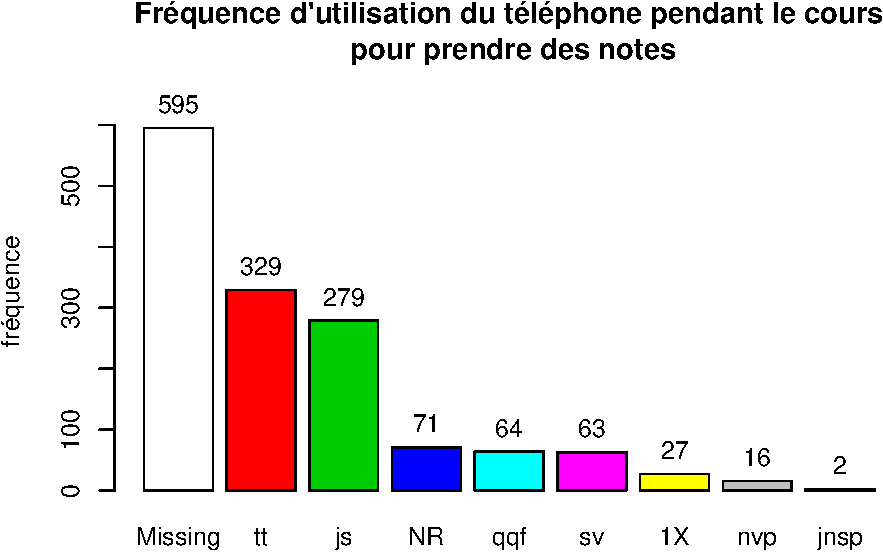
\includegraphics{qs_etudiants_files/figure-latex/utilisatin3-1.pdf}

\begin{verbatim}
as.factor(d1$Q8) : 
        Frequency   %(NA+)   %(NA-)
NA's          595     41.1      0.0
tt            329     22.8     38.7
js            279     19.3     32.8
NR             71      4.9      8.3
qqf            64      4.4      7.5
sv             63      4.4      7.4
1X             27      1.9      3.2
nvp            16      1.1      1.9
jnsp            2      0.1      0.2
  Total      1446    100.0    100.0
\end{verbatim}

\subsection{Q9- A quelle fréquence, avez-vous utilisé votre tablette,
et/ ou votre ordinateur PENDANT ce cours (en dehors des temps de pause
éventuels) pour faire autre chose que prendre des notes ou chercher sur
internet des informations au sujet du cours
?}\label{q9--a-quelle-frequence-avez-vous-utilise-votre-tablette-et-ou-votre-ordinateur-pendant-ce-cours-en-dehors-des-temps-de-pause-eventuels-pour-faire-autre-chose-que-prendre-des-notes-ou-chercher-sur-internet-des-informations-au-sujet-du-cours}

question 50

\begin{figure}[htbp]
\centering
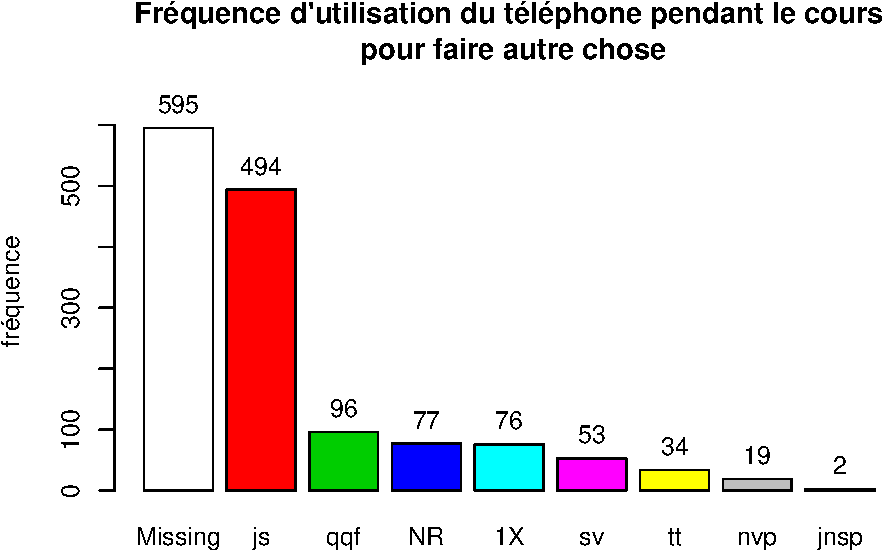
\includegraphics{qs_etudiants_files/figure-latex/utilisation4-1.pdf}
\end{figure}

\begin{verbatim}
as.factor(d1$Q9) : 
        Frequency   %(NA+)   %(NA-)
NA's          595     41.1      0.0
js            494     34.2     58.0
qqf            96      6.6     11.3
NR             77      5.3      9.0
1X             76      5.3      8.9
sv             53      3.7      6.2
tt             34      2.4      4.0
nvp            19      1.3      2.2
jnsp            2      0.1      0.2
  Total      1446    100.0    100.0
\end{verbatim}

\section{Questions supplémentaires}\label{questions-supplementaires}

\begin{itemize}
\itemsep1pt\parskip0pt\parsep0pt
\item
  Est-ce que les comportements concernant en particulier la prise de
  notes étaient différents lorsque les étudiants n'avaient pas de
  support et savaient qu'ils ne l'auraient jamais à autrement dit,
  est-ce que l'utilisation des outils numériques est modifiée selon que
  les étudiants aient ou non accès à un support de cours ? comparaison
  de la population (HUS 1, E1, C2, C3, B1, B2) avec (Sa1, SV1 SV2, H1
  H2, HUS 2 HUS 3, C1,) sur Q4 et Q7 Est-ce possible .?
\end{itemize}

\section{Résultats selon la
promotion}\label{resultats-selon-la-promotion}

On crée une variable supplémentaire PROMO:

\begin{verbatim}
##  p1  p2  p3 
## 568 365 513
\end{verbatim}

p = propmotion, chiffre = année

Comparaison 1ère année (S1 + S2), 2ème année (S3 + S4), 3ème année (S5 +
S6) comparaison de la population( HUS1, SV1, C2, B2, et M1) avec (HUS3,
H1, E1, C1) avec (Sa1, SV2, HUS2 , C3, H2, B1 et M2) sur Q4 et Q7.

\subsection{Question Q4}\label{question-q4}

La queestion 4 comporte 16 sous questions dichotomiques, correspondant
aux colonnes 15 à 30. Il faut éliminer la colonne 27 qui contient du
texte libre. Enfin on ajoute les colonnes 52 (age) et 53 (promotion)
pour une analyse en sous-groupes. Au final le dataframe q4 comporte 15
colonnes dichotomiqes + 2 colonnes servant à fabriquer des sous-groupes.

\begin{verbatim}
       p1  p2  p3
Q4.1   83  45  68
Q4.2   80  53 137
Q4.3   13   6   6
Q4.4  340 162 326
Q4.5  125  51 200
Q4.6    3   1   1
Q4.7   13   7  13
Q4.8  101  51 120
Q4.9   28  15  19
Q4.10  79  44 104
Q4.11  36   8  20
Q4.12 144  62 124
Q4.14 132 125  83
Q4.15  22  27  18
Q4.16   6   2   0
\end{verbatim}

suite: comparaison des 3 groupes pour chaque sous-question par test chi2
après transformation des NA en `0'.

\begin{verbatim}
   0    1 
1250  196 
\end{verbatim}

\begin{verbatim}
   
q    p1  p2  p3
  0 485 320 445
  1  83  45  68
\end{verbatim}

\begin{verbatim}

    Pearson's Chi-squared test

data:  table(q, q4$PROMO)
X-squared = 1.05, df = 2, p-value = 0.5916
\end{verbatim}

\begin{verbatim}
   
q    p1  p2  p3
  0 485 320 445
  1  83  45  68
\end{verbatim}

\begin{verbatim}
   
q          p1        p2        p3
  0 491.00968 315.52559 443.46473
  1  76.99032  49.47441  69.53527
\end{verbatim}

Alternative avec le test \textbf{prop.test}. La ligne \emph{sample
estimate} donne la proportion de `non' dans chaque promotion.

\begin{verbatim}

    3-sample test for equality of proportions without continuity
    correction

data:  t(table(q, q4$PROMO))
X-squared = 1.05, df = 2, p-value = 0.5916
alternative hypothesis: two.sided
sample estimates:
   prop 1    prop 2    prop 3 
0.8538732 0.8767123 0.8674464 
\end{verbatim}

A la question \emph{chercher sur internet des informations qui me
manquaient au sujet du cours}, il n'y a pas de différence de
comportement entre les propmotions.

Pour chacune des 15 sous-questions on compare les réponses de 3
promotions par un test du chi2. Si \textbf{p-value} est supérieur à
0.05, alors il n'y a pas de différence de comportement entre les
promotions pour cette sous-question. Dans la cas contraire, au moins une
promotion ne se comporte pas comme les autres:

\begin{verbatim}
[1] "Q4.1"

    Pearson's Chi-squared test

data:  table(q, q4$PROMO)
X-squared = 1.05, df = 2, p-value = 0.5916

[1] "Q4.2"

    Pearson's Chi-squared test

data:  table(q, q4$PROMO)
X-squared = 33.8167, df = 2, p-value = 0.00000004537

[1] "Q4.3"

    Pearson's Chi-squared test

data:  table(q, q4$PROMO)
X-squared = 2.0079, df = 2, p-value = 0.3664

[1] "Q4.4"

    Pearson's Chi-squared test

data:  table(q, q4$PROMO)
X-squared = 34.5843, df = 2, p-value = 0.00000003091

[1] "Q4.5"

    Pearson's Chi-squared test

data:  table(q, q4$PROMO)
X-squared = 77.1108, df = 2, p-value < 2.2e-16
\end{verbatim}

\begin{verbatim}
Warning in chisq.test(table(q, q4$PROMO)): Chi-squared approximation may be
incorrect
\end{verbatim}

\begin{verbatim}
[1] "Q4.6"

    Pearson's Chi-squared test

data:  table(q, q4$PROMO)
X-squared = 0.9417, df = 2, p-value = 0.6245

[1] "Q4.7"

    Pearson's Chi-squared test

data:  table(q, q4$PROMO)
X-squared = 0.3634, df = 2, p-value = 0.8338

[1] "Q4.8"

    Pearson's Chi-squared test

data:  table(q, q4$PROMO)
X-squared = 13.0376, df = 2, p-value = 0.001475

[1] "Q4.9"

    Pearson's Chi-squared test

data:  table(q, q4$PROMO)
X-squared = 1.0248, df = 2, p-value = 0.5991

[1] "Q4.10"

    Pearson's Chi-squared test

data:  table(q, q4$PROMO)
X-squared = 13.1483, df = 2, p-value = 0.001396

[1] "Q4.11"

    Pearson's Chi-squared test

data:  table(q, q4$PROMO)
X-squared = 9.5534, df = 2, p-value = 0.008424

[1] "Q4.12"

    Pearson's Chi-squared test

data:  table(q, q4$PROMO)
X-squared = 9.6521, df = 2, p-value = 0.008018

[1] "Q4.14"

    Pearson's Chi-squared test

data:  table(q, q4$PROMO)
X-squared = 38.7471, df = 2, p-value = 0.000000003856

[1] "Q4.15"

    Pearson's Chi-squared test

data:  table(q, q4$PROMO)
X-squared = 8.521, df = 2, p-value = 0.01411
\end{verbatim}

\begin{verbatim}
Warning in chisq.test(table(q, q4$PROMO)): Chi-squared approximation may be
incorrect
\end{verbatim}

\begin{verbatim}
[1] "Q4.16"

    Pearson's Chi-squared test

data:  table(q, q4$PROMO)
X-squared = 5.4671, df = 2, p-value = 0.06499
\end{verbatim}

Même analyse en utilisant le \textbf{test exact de Fisher} qui donne un
résultat plus précis que la chi2 en cas d'effectifs faibles:

\begin{verbatim}
[1] "Q4.1"

    Fisher's Exact Test for Count Data

data:  table(q, q4$PROMO)
p-value = 0.6038
alternative hypothesis: two.sided

[1] "Q4.2"

    Fisher's Exact Test for Count Data

data:  table(q, q4$PROMO)
p-value = 0.00000008304
alternative hypothesis: two.sided

[1] "Q4.3"

    Fisher's Exact Test for Count Data

data:  table(q, q4$PROMO)
p-value = 0.3576
alternative hypothesis: two.sided

[1] "Q4.4"

    Fisher's Exact Test for Count Data

data:  table(q, q4$PROMO)
p-value = 0.00000003458
alternative hypothesis: two.sided

[1] "Q4.5"

    Fisher's Exact Test for Count Data

data:  table(q, q4$PROMO)
p-value < 2.2e-16
alternative hypothesis: two.sided

[1] "Q4.6"

    Fisher's Exact Test for Count Data

data:  table(q, q4$PROMO)
p-value = 0.8525
alternative hypothesis: two.sided

[1] "Q4.7"

    Fisher's Exact Test for Count Data

data:  table(q, q4$PROMO)
p-value = 0.8561
alternative hypothesis: two.sided

[1] "Q4.8"

    Fisher's Exact Test for Count Data

data:  table(q, q4$PROMO)
p-value = 0.001524
alternative hypothesis: two.sided

[1] "Q4.9"

    Fisher's Exact Test for Count Data

data:  table(q, q4$PROMO)
p-value = 0.6171
alternative hypothesis: two.sided

[1] "Q4.10"

    Fisher's Exact Test for Count Data

data:  table(q, q4$PROMO)
p-value = 0.00164
alternative hypothesis: two.sided

[1] "Q4.11"

    Fisher's Exact Test for Count Data

data:  table(q, q4$PROMO)
p-value = 0.007551
alternative hypothesis: two.sided

[1] "Q4.12"

    Fisher's Exact Test for Count Data

data:  table(q, q4$PROMO)
p-value = 0.006745
alternative hypothesis: two.sided

[1] "Q4.14"

    Fisher's Exact Test for Count Data

data:  table(q, q4$PROMO)
p-value = 0.000000005307
alternative hypothesis: two.sided

[1] "Q4.15"

    Fisher's Exact Test for Count Data

data:  table(q, q4$PROMO)
p-value = 0.01968
alternative hypothesis: two.sided

[1] "Q4.16"

    Fisher's Exact Test for Count Data

data:  table(q, q4$PROMO)
p-value = 0.04104
alternative hypothesis: two.sided
\end{verbatim}

\textbf{Ne pas tenir compte de cette remarque}

Modèle plus complexe (utilité ?).
\href{http://cran.r-project.org/doc/contrib/Herve-Aide-memoire-statistique.pdf}{Référence}
fiche 61 et 62.

\begin{Shaded}
\begin{Highlighting}[]
\CommentTok{# f <- glm(q1 ~ q4$PROMO, family = "binomial")}
\CommentTok{# f}
\CommentTok{# summary(f)}
\end{Highlighting}
\end{Shaded}

\subsection{Question Q7}\label{question-q7}

La question 7 comporte 15 sous questions de Q7.1 à Q7.16 (colonnes 33 à
48). On retire la colonne 13 qui est du texte libre. On ajoute la
colonne PROMO (promotion) pour l'analyse en sous-groupe.

\begin{verbatim}
       p1  p2  p3
Q7.1   22  18  23
Q7.2   19  10  26
Q7.3   13   6  20
Q7.4   25   7  38
Q7.5    0   2   5
Q7.6    3   1   1
Q7.7   17   6  19
Q7.8    2   2   1
Q7.9   22   6  14
Q7.10  24  30  37
Q7.11 191  89  88
Q7.12  28  18   7
Q7.14  86  72  76
Q7.15 252 129 259
Q7.16   9   4   1
\end{verbatim}

\textbf{REMARQUE}: les lignes pour lesquelles un des effectif est
inférieur à 5 donnent des résultats douteux au test du chi2.

Pour chacune des 15 sous-questions on compare les réponses de 3
promotions par un test du chi2. Si \textbf{p-value} est supérieur à
0.05, alors il n'y a pas de différence de comportement entre les
promotions pour cette sous-question. Dans la cas contraire, au moins une
promotion ne se comporte pas comme les autres:

\begin{verbatim}
[1] "Q7.1"

    Pearson's Chi-squared test

data:  table(q, q7$PROMO)
X-squared = 0.6278, df = 2, p-value = 0.7306

[1] "Q7.2"

    Pearson's Chi-squared test

data:  table(q, q7$PROMO)
X-squared = 3.6977, df = 2, p-value = 0.1574

[1] "Q7.3"

    Pearson's Chi-squared test

data:  table(q, q7$PROMO)
X-squared = 4.7259, df = 2, p-value = 0.09414

[1] "Q7.4"

    Pearson's Chi-squared test

data:  table(q, q7$PROMO)
X-squared = 14.3437, df = 2, p-value = 0.0007679
\end{verbatim}

\begin{verbatim}
Warning in chisq.test(table(q, q7$PROMO)): Chi-squared approximation may be
incorrect
\end{verbatim}

\begin{verbatim}
[1] "Q7.5"

    Pearson's Chi-squared test

data:  table(q, q7$PROMO)
X-squared = 5.3566, df = 2, p-value = 0.06868
\end{verbatim}

\begin{verbatim}
Warning in chisq.test(table(q, q7$PROMO)): Chi-squared approximation may be
incorrect
\end{verbatim}

\begin{verbatim}
[1] "Q7.6"

    Pearson's Chi-squared test

data:  table(q, q7$PROMO)
X-squared = 0.9417, df = 2, p-value = 0.6245

[1] "Q7.7"

    Pearson's Chi-squared test

data:  table(q, q7$PROMO)
X-squared = 3.2345, df = 2, p-value = 0.1984
\end{verbatim}

\begin{verbatim}
Warning in chisq.test(table(q, q7$PROMO)): Chi-squared approximation may be
incorrect
\end{verbatim}

\begin{verbatim}
[1] "Q7.8"

    Pearson's Chi-squared test

data:  table(q, q7$PROMO)
X-squared = 0.7723, df = 2, p-value = 0.6797

[1] "Q7.9"

    Pearson's Chi-squared test

data:  table(q, q7$PROMO)
X-squared = 4.003, df = 2, p-value = 0.1351

[1] "Q7.10"

    Pearson's Chi-squared test

data:  table(q, q7$PROMO)
X-squared = 7.1495, df = 2, p-value = 0.02802

[1] "Q7.11"

    Pearson's Chi-squared test

data:  table(q, q7$PROMO)
X-squared = 38.8441, df = 2, p-value = 0.000000003674

[1] "Q7.12"

    Pearson's Chi-squared test

data:  table(q, q7$PROMO)
X-squared = 11.9195, df = 2, p-value = 0.002581

[1] "Q7.14"

    Pearson's Chi-squared test

data:  table(q, q7$PROMO)
X-squared = 4.5408, df = 2, p-value = 0.1033

[1] "Q7.15"

    Pearson's Chi-squared test

data:  table(q, q7$PROMO)
X-squared = 19.8318, df = 2, p-value = 0.00004938
\end{verbatim}

\begin{verbatim}
Warning in chisq.test(table(q, q7$PROMO)): Chi-squared approximation may be
incorrect
\end{verbatim}

\begin{verbatim}
[1] "Q7.16"

    Pearson's Chi-squared test

data:  table(q, q7$PROMO)
X-squared = 5.5114, df = 2, p-value = 0.06356
\end{verbatim}

Même analyse en utilisant le \textbf{test exact de Fisher} qui donne un
résultat plus précis que la chi2 en cas d'effectifs faibles:

\begin{verbatim}
[1] "Q7.1"

    Fisher's Exact Test for Count Data

data:  table(q, q7$PROMO)
p-value = 0.7252
alternative hypothesis: two.sided

[1] "Q7.2"

    Fisher's Exact Test for Count Data

data:  table(q, q7$PROMO)
p-value = 0.1851
alternative hypothesis: two.sided

[1] "Q7.3"

    Fisher's Exact Test for Count Data

data:  table(q, q7$PROMO)
p-value = 0.11
alternative hypothesis: two.sided

[1] "Q7.4"

    Fisher's Exact Test for Count Data

data:  table(q, q7$PROMO)
p-value = 0.000556
alternative hypothesis: two.sided

[1] "Q7.5"

    Fisher's Exact Test for Count Data

data:  table(q, q7$PROMO)
p-value = 0.04439
alternative hypothesis: two.sided

[1] "Q7.6"

    Fisher's Exact Test for Count Data

data:  table(q, q7$PROMO)
p-value = 0.8525
alternative hypothesis: two.sided

[1] "Q7.7"

    Fisher's Exact Test for Count Data

data:  table(q, q7$PROMO)
p-value = 0.193
alternative hypothesis: two.sided

[1] "Q7.8"

    Fisher's Exact Test for Count Data

data:  table(q, q7$PROMO)
p-value = 0.7437
alternative hypothesis: two.sided

[1] "Q7.9"

    Fisher's Exact Test for Count Data

data:  table(q, q7$PROMO)
p-value = 0.1436
alternative hypothesis: two.sided

[1] "Q7.10"

    Fisher's Exact Test for Count Data

data:  table(q, q7$PROMO)
p-value = 0.02268
alternative hypothesis: two.sided

[1] "Q7.11"

    Fisher's Exact Test for Count Data

data:  table(q, q7$PROMO)
p-value = 0.000000003063
alternative hypothesis: two.sided

[1] "Q7.12"

    Fisher's Exact Test for Count Data

data:  table(q, q7$PROMO)
p-value = 0.001148
alternative hypothesis: two.sided

[1] "Q7.14"

    Fisher's Exact Test for Count Data

data:  table(q, q7$PROMO)
p-value = 0.1091
alternative hypothesis: two.sided

[1] "Q7.15"

    Fisher's Exact Test for Count Data

data:  table(q, q7$PROMO)
p-value = 0.00004577
alternative hypothesis: two.sided

[1] "Q7.16"

    Fisher's Exact Test for Count Data

data:  table(q, q7$PROMO)
p-value = 0.04678
alternative hypothesis: two.sided
\end{verbatim}

\section{Accès WIFI}\label{acces-wifi}

Est-ce que le fait d'avoir accès à la WIFI modifie l'usage de
l'ordinateur ou de la tablette, et en particulier leur usage à des fins
ne relevant pas de l'apprentissage en lien avec le cours comparaison des
étudiants ayant répondu ot ou osp à tablette et ordi et appartenant d'un
côté au group (SV1 sv2 Sa1 M1 M2 E1 B1 et B2) par rapport au groupe (
HUS1 HUS 2 HUS3 H1 H2 C1 C2C3 ) sur la question 7

\begin{verbatim}
## Groupe1 Groupe2 
##     629     817
\end{verbatim}

La question 7 comporte 15 sous questions de Q7.1 à Q7.16 (colonnes 33 à
48). On retire la colonne 13 qui est du texte libre. On ajoute la
colonne PROMO2 (promotion) pour l'analyse en sous-groupe.

\begin{verbatim}
      Groupe1 Groupe2
Q7.1       35      28
Q7.2       32      23
Q7.3       24      15
Q7.4       53      17
Q7.5        3       4
Q7.6        4       1
Q7.7       23      19
Q7.8        2       3
Q7.9       27      15
Q7.10      39      52
Q7.11     138     230
Q7.12      20      33
Q7.14      99     135
Q7.15     280     360
Q7.16       5       9
\end{verbatim}

\textbf{REMARQUE}: les lignes pour lesquelles un des effectif est
inférieur à 5 donnent des résultats douteux au test du chi2.

Pour chacune des 15 sous-questions on compare les réponses de 2 groupes
par un test du chi2. Si \textbf{p-value} est supérieur à 0.05, alors il
n'y a pas de différence de comportement entre les promotions pour cette
sous-question. Dans la cas contraire, au moins une promotion ne se
comporte pas comme les autres:

\begin{verbatim}
[1] "Q7.1"

    Pearson's Chi-squared test with Yates' continuity correction

data:  table(q, q7$PROMO)
X-squared = 3.3996, df = 1, p-value = 0.06521

[1] "Q7.2"

    Pearson's Chi-squared test with Yates' continuity correction

data:  table(q, q7$PROMO)
X-squared = 4.4132, df = 1, p-value = 0.03566

[1] "Q7.3"

    Pearson's Chi-squared test with Yates' continuity correction

data:  table(q, q7$PROMO)
X-squared = 4.5793, df = 1, p-value = 0.03236

[1] "Q7.4"

    Pearson's Chi-squared test with Yates' continuity correction

data:  table(q, q7$PROMO)
X-squared = 29.6997, df = 1, p-value = 0.00000005044
\end{verbatim}

\begin{verbatim}
Warning in chisq.test(table(q, q7$PROMO)): Chi-squared approximation may be
incorrect
\end{verbatim}

\begin{verbatim}
[1] "Q7.5"

    Pearson's Chi-squared test with Yates' continuity correction

data:  table(q, q7$PROMO)
X-squared = 0, df = 1, p-value = 1
\end{verbatim}

\begin{verbatim}
Warning in chisq.test(table(q, q7$PROMO)): Chi-squared approximation may be
incorrect
\end{verbatim}

\begin{verbatim}
[1] "Q7.6"

    Pearson's Chi-squared test with Yates' continuity correction

data:  table(q, q7$PROMO)
X-squared = 1.4337, df = 1, p-value = 0.2312

[1] "Q7.7"

    Pearson's Chi-squared test with Yates' continuity correction

data:  table(q, q7$PROMO)
X-squared = 1.7855, df = 1, p-value = 0.1815
\end{verbatim}

\begin{verbatim}
Warning in chisq.test(table(q, q7$PROMO)): Chi-squared approximation may be
incorrect
\end{verbatim}

\begin{verbatim}
[1] "Q7.8"

    Pearson's Chi-squared test with Yates' continuity correction

data:  table(q, q7$PROMO)
X-squared = 0, df = 1, p-value = 1

[1] "Q7.9"

    Pearson's Chi-squared test with Yates' continuity correction

data:  table(q, q7$PROMO)
X-squared = 6.7584, df = 1, p-value = 0.009331

[1] "Q7.10"

    Pearson's Chi-squared test with Yates' continuity correction

data:  table(q, q7$PROMO)
X-squared = 0.0003, df = 1, p-value = 0.9853

[1] "Q7.11"

    Pearson's Chi-squared test with Yates' continuity correction

data:  table(q, q7$PROMO)
X-squared = 6.905, df = 1, p-value = 0.008595

[1] "Q7.12"

    Pearson's Chi-squared test with Yates' continuity correction

data:  table(q, q7$PROMO)
X-squared = 0.5201, df = 1, p-value = 0.4708

[1] "Q7.14"

    Pearson's Chi-squared test with Yates' continuity correction

data:  table(q, q7$PROMO)
X-squared = 0.1086, df = 1, p-value = 0.7417

[1] "Q7.15"

    Pearson's Chi-squared test with Yates' continuity correction

data:  table(q, q7$PROMO)
X-squared = 0.0139, df = 1, p-value = 0.9061

[1] "Q7.16"

    Pearson's Chi-squared test with Yates' continuity correction

data:  table(q, q7$PROMO)
X-squared = 0.1021, df = 1, p-value = 0.7493
\end{verbatim}

Même analyse en utilisant le \textbf{test exact de Fisher} qui donne un
résultat plus précis que la chi2 en cas d'effectifs faibles:

\begin{verbatim}
[1] "Q7.1"

    Fisher's Exact Test for Count Data

data:  table(q, q7$PROMO)
p-value = 0.05188
alternative hypothesis: true odds ratio is not equal to 1
95 percent confidence interval:
 0.3487933 1.0321911
sample estimates:
odds ratio 
 0.6025082 

[1] "Q7.2"

    Fisher's Exact Test for Count Data

data:  table(q, q7$PROMO)
p-value = 0.02691
alternative hypothesis: true odds ratio is not equal to 1
95 percent confidence interval:
 0.2987513 0.9644285
sample estimates:
odds ratio 
 0.5406644 

[1] "Q7.3"

    Fisher's Exact Test for Count Data

data:  table(q, q7$PROMO)
p-value = 0.03198
alternative hypothesis: true odds ratio is not equal to 1
95 percent confidence interval:
 0.2280039 0.9460479
sample estimates:
odds ratio 
 0.4717196 

[1] "Q7.4"

    Fisher's Exact Test for Count Data

data:  table(q, q7$PROMO)
p-value = 0.00000003769
alternative hypothesis: true odds ratio is not equal to 1
95 percent confidence interval:
 0.1241147 0.4106147
sample estimates:
odds ratio 
 0.2311688 

[1] "Q7.5"

    Fisher's Exact Test for Count Data

data:  table(q, q7$PROMO)
p-value = 1
alternative hypothesis: true odds ratio is not equal to 1
95 percent confidence interval:
 0.1729835 7.0344121
sample estimates:
odds ratio 
  1.026634 

[1] "Q7.6"

    Fisher's Exact Test for Count Data

data:  table(q, q7$PROMO)
p-value = 0.1736
alternative hypothesis: true odds ratio is not equal to 1
95 percent confidence interval:
 0.003888542 1.943188489
sample estimates:
odds ratio 
 0.1916576 

[1] "Q7.7"

    Fisher's Exact Test for Count Data

data:  table(q, q7$PROMO)
p-value = 0.1556
alternative hypothesis: true odds ratio is not equal to 1
95 percent confidence interval:
 0.3199895 1.2169580
sample estimates:
odds ratio 
 0.6275462 

[1] "Q7.8"

    Fisher's Exact Test for Count Data

data:  table(q, q7$PROMO)
p-value = 1
alternative hypothesis: true odds ratio is not equal to 1
95 percent confidence interval:
  0.1319202 13.8763590
sample estimates:
odds ratio 
  1.155273 

[1] "Q7.9"

    Fisher's Exact Test for Count Data

data:  table(q, q7$PROMO)
p-value = 0.006924
alternative hypothesis: true odds ratio is not equal to 1
95 percent confidence interval:
 0.2044110 0.8210999
sample estimates:
odds ratio 
 0.4172633 

[1] "Q7.10"

    Fisher's Exact Test for Count Data

data:  table(q, q7$PROMO)
p-value = 0.9136
alternative hypothesis: true odds ratio is not equal to 1
95 percent confidence interval:
 0.6559991 1.6232148
sample estimates:
odds ratio 
  1.028306 

[1] "Q7.11"

    Fisher's Exact Test for Count Data

data:  table(q, q7$PROMO)
p-value = 0.007392
alternative hypothesis: true odds ratio is not equal to 1
95 percent confidence interval:
 1.086410 1.792038
sample estimates:
odds ratio 
  1.393768 

[1] "Q7.12"

    Fisher's Exact Test for Count Data

data:  table(q, q7$PROMO)
p-value = 0.4017
alternative hypothesis: true odds ratio is not equal to 1
95 percent confidence interval:
 0.7058042 2.3818660
sample estimates:
odds ratio 
  1.281479 

[1] "Q7.14"

    Fisher's Exact Test for Count Data

data:  table(q, q7$PROMO)
p-value = 0.719
alternative hypothesis: true odds ratio is not equal to 1
95 percent confidence interval:
 0.7911582 1.4227132
sample estimates:
odds ratio 
  1.059694 

[1] "Q7.15"

    Fisher's Exact Test for Count Data

data:  table(q, q7$PROMO)
p-value = 0.8728
alternative hypothesis: true odds ratio is not equal to 1
95 percent confidence interval:
 0.7921136 1.2173051
sample estimates:
odds ratio 
 0.9818764 

[1] "Q7.16"

    Fisher's Exact Test for Count Data

data:  table(q, q7$PROMO)
p-value = 0.6011
alternative hypothesis: true odds ratio is not equal to 1
95 percent confidence interval:
 0.4158249 5.3060086
sample estimates:
odds ratio 
   1.38979 
\end{verbatim}

\begin{center}\rule{3in}{0.4pt}\end{center}

Est-ce que ceux qui avaient leur téléphone ou leur smartphone sur la
table l'ont plus utilisé que ceux qui l'avaient dans leur sac, et pour
faire quoi ? quelque soit la génération

Cela revient à croiser Q3 et Q4 qui comportent respectivement 4 et 16
sous question chacune ayant 2 à plusieurs modalités. Temps de travail 3
à 4 heures.

\section{Information de session}\label{information-de-session}

Informations pour le chapitre matériel et méthode.

\begin{verbatim}
R version 3.1.3 (2015-03-09)
Platform: x86_64-apple-darwin13.4.0 (64-bit)
Running under: OS X 10.10.3 (Yosemite)

locale:
[1] fr_FR.UTF-8/fr_FR.UTF-8/fr_FR.UTF-8/C/fr_FR.UTF-8/fr_FR.UTF-8

attached base packages:
[1] stats     graphics  grDevices utils     datasets  methods   base     

other attached packages:
[1] knitr_1.10.5     xtable_1.7-4     stringr_1.0.0    epicalc_2.15.1.0
[5] nnet_7.3-9       MASS_7.3-41      survival_2.38-2  foreign_0.8-63  

loaded via a namespace (and not attached):
 [1] digest_0.6.8    evaluate_0.7    formatR_1.2     htmltools_0.2.6
 [5] magrittr_1.5    rmarkdown_0.7   splines_3.1.3   stringi_0.4-1  
 [9] tools_3.1.3     yaml_2.1.13    
\end{verbatim}

\begin{verbatim}

To cite R in publications use:

  R Core Team (2015). R: A language and environment for
  statistical computing. R Foundation for Statistical Computing,
  Vienna, Austria. URL http://www.R-project.org/.

A BibTeX entry for LaTeX users is

  @Manual{,
    title = {R: A Language and Environment for Statistical Computing},
    author = {{R Core Team}},
    organization = {R Foundation for Statistical Computing},
    address = {Vienna, Austria},
    year = {2015},
    url = {http://www.R-project.org/},
  }

We have invested a lot of time and effort in creating R, please
cite it when using it for data analysis. See also
'citation("pkgname")' for citing R packages.
\end{verbatim}

\end{document}
